\documentclass{article}
% if you need to pass options to natbib, use, e.g.:
%     \PassOptionsToPackage{numbers, compress}{natbib}
% before loading neurips_2023


% ready for submission
\usepackage[preprint]{neurips_2023}


% to compile a preprint version, e.g., for submission to arXiv, add add the
% [preprint] option:
%     \usepackage[preprint]{neurips_2023}


% to compile a camera-ready version, add the [final] option, e.g.:
%     \usepackage[final]{neurips_2023}


% to avoid loading the natbib package, add option nonatbib:
%    \usepackage[nonatbib]{neurips_2023}

\usepackage{amsmath}
\usepackage{graphicx}
\usepackage{caption}
\usepackage{float}
\usepackage[utf8]{inputenc} % allow utf-8 input
\usepackage[T1]{fontenc}    % use 8-bit T1 fonts
\usepackage{hyperref}       % hyperlinks
\usepackage{url}            % simple URL typesetting
\usepackage{booktabs}       % professional-quality tables
\usepackage{amsfonts}       % blackboard math symbols
\usepackage{nicefrac}       % compact symbols for 1/2, etc.
\usepackage{microtype}      % microtypography
\usepackage{xcolor}
\usepackage{cleveref}         % colors

\title{Machine Learning Project Report}

\author{
    Jop Zitman 2023280072\\
    Department of Computer Science\\
    Tsinghua University\\
    Beijing, China \\
    \texttt{lilw23@mails.tsinghua.edu.cn} \\
    \And
    Lauriane Teyssier 2023280008\\
    Department of Computer Science\\
    Tsinghua University\\
    Beijing, China \\
    \texttt{yell23@mails.tsinghua.edu.cn} \\
}

% Document
\begin{document}

    \maketitle

    \begin{abstract}
        The abstract paragraph should be indented \nicefrac{1}{2}~inch (3~picas) on
        both the left- and right-hand margins.
        Use 10~point type, with a vertical
        spacing (leading) of 11~points.
        The word \textbf{Abstract} must be centered,
        bold, and in point size 12.
        Two line spaces precede the abstract.
        The abstract must be limited to one paragraph.
    \end{abstract}

    \newpage
    \tableofcontents
    \newpage


%    \section{Jop dump}
%
%    https://www.kaggle.com/datasets/shawon10/url-classification-dataset-dmoz/data
%    https://utatds.github.io/2017-01-18-URL-classification-using-DMOZ-data/
%    https://github.com/stanfordnlp/GloVe
%    https://spotintelligence.com/2023/02/15/word2vec-for-text-classification/
%    https://huggingface.co/elftsdmr/malware-url-detect


    \section{Problem description and motivation}\label{sec:problem-description-and-motivation}
%    What’s the background of the problem?
%    Is it theory-driven, or deeply rooted in some useful application situations?
%    Is it important or necessary?
%    What impact will it bring if you finally solve it?

    The motivation for using machine learning to classify phishing URLs gains urgency against the backdrop of an alarming rise in cyber threats.
    Phishing, a deceptive practice where attackers pose as legitimate entities to harvest sensitive information, has not only intensified in sophistication but also in frequency.
    The Anti-Phishing Working Group's (APWG) report for the fourth quarter of 2022 provides a stark illustration: over 4.7 million phishing attacks were recorded in 2022, marking a year-over-year increase exceeding 150\% \cite{PhishingActivityTrendsReport}.
    The final quarter of that year alone witnessed 1,350,037 attacks, slightly up from the previous quarter's record of 1,270,883 incidents, indicating a persistent and escalating threat.

    The financial sector bore the brunt of these attacks, accounting for 27.7\% of all phishing incidents.
    Phishing attempts against webmail and software-as-a-service (SAAS) providers were also notable, comprising 17.7\% of the attacks.
    These attacks, which involve impersonating trusted parties to manipulate victims into transferring funds or revealing sensitive data, have led to losses in the billions.
    In the fourth quarter of 2022 alone, the average amount requested in wire transfer BEC attacks soared to \$132,559, marking a 41\% increase from the previous quarter.

    In addition, the FBI’s Internet Crime Complaint Center reported a near doubling of phishing incidents from 2019 to 2020, resulting in substantial financial losses.

    The methods employed in these attacks are diverse.
    The fourth quarter of 2022 saw advance fee fraud scams surpassing gift card requests as the most popular method, accounting for 39\% of all attacks. This shift underscores the adaptability and evolving strategies of attackers. Gift cards, particularly Amazon and Apple cards, remained popular among scammers, with 60\% favoring Amazon cards.

    Historically, phishing attempts were more transparent and easier to spot due to their general approach and clear warning signs.
    However, the integration of AI has led to more subtle and customized phishing strategies, using personal information to boost their believability.
    This shift calls for a detection system that is both intelligent and adaptive, capable of keeping pace with these evolving threats.

    Today's method of detecting phishing URLs is to rely on blacklists, which are lists of known phishing URLs.

    This landscape of escalating and evolving phishing attacks underscores the critical need for advanced detection methods, including the application of machine learning for phishing URL classification.

%    TODO Statistics on how much money phishing represents nowadays


    \section{Related works}\label{sec:related-works}

    In the realm of URL-based phishing detection, a rich literature addresses each part of the detection process, from the creation of set of databases to comparison metrics between the methodologies, including comparison of classification algorithm or data pre-processing.
    The approach can be divided into two main groups, the authors focusing on Machine Learning and and those proposing an approach based on deep learning.
    We will highlight references of both approaches.

    \subsection{Machine Learning based approaches}\label{subsec:machine-learning-based-approaches}

    \begin{itemize}

        \item An phishing URL detection method (\cite{PhishingURLDetection}) compares different Machine Learning classification algorithm.
        Their data processing involves first the detection of words through 17 NLP handcrafted features.
        It then relies on a Markov Chain Model to identify random word.
        The classification is based on detecting Typosquatting and employs various algorithms like Naive Bayes, Random Forest, kNN, Adaboost, K-star, SMO, and Decision Tree.
        The study reached 97.20\% of accuracy with Weka's RFC (Random Forest Classifier) on a 10\% sub-sample from the Ebbu2017 dataset.

        \item In their paper\cite{PhishSafe}, Jain and Gupta developed an anti-phishing system employing 14 handcrafted URL descriptors.
        They conducted tests using two classifiers: Naive Bayes, which achieved an accuracy of 76.87\%, and Support Vector Machine, demonstrating a higher accuracy of 91.28\%.

        \item The study presented in\cite{LexicalFeatureSelection} implemented a classification system based on lexical features extracted from URLs. Their methodology involved a feature extraction from URLs, the selection of the most relevant features through chi-square feature selection, and the utilization of various machine learning algorithms for classification.
        With nine selected features and a Random Forest (RF) classifier, they achieved their best accuracy of 98.57%.

    \end{itemize}

    \subsection{Deep Learning based approaches}\label{subsec:deep-learning-based-approaches}

    \begin{itemize}
        \item  The Spanish national institute for security classifies in\cite{PhishingLoginURLDetection} login form URLs into malicious or legitimate categories through two distinct techniques.
        The first technique employs machine learning with text pre-processing, including symbol-based word separation, text conversion into feature vectors (use 38 features, among them the frequency of symbols, the number of digits, length, \ldots), and classification.
        Eight different classifiers have been used for comparison.
        The second technique utilizes deep learning, specifically a convolutional neural network, with no text preprocessing.
        The results show that the best performance is archived for the machine learning NLP frequency feature extraction combined with Logistic Regression (accuracy of 96.50\%).


        \item \cite{EfficientDeepLearningPhishingDetection} introduced three Deep Learning models for classifying phishing URLs, utilizing ten of the most relevant handcrafted features out of a total of 18, which included characteristics like the number of dots, length, and the presence of HTTPS. These models included Convolutional Neural Network (CNN), Deep Neural Network (DNN), and Long Short-Term Memory (LSTM). Among these, the LSTM model achieved the best performance, boasting an impressive accuracy of 99.57\%.

        \item An RCNN model to classify phishing URLs is compared with different machine learning common approaches (Naïves Bayes, Logistic Regression, random forest and XGBoost) on four different types of features (hand crafted, character embedding, character level TF-IDF and character level count vector features)\cite{CharacterLevelCNN}.
        The URL is used as input for a tokenizer and then then transformed into a matrix using one-hot encoding.
        Their RCNN model obtained 95:02\% accuracy.

    \end{itemize}

    \subsection{Large Language Models}\label{subsec:large-language-models}
    PhishBert~\cite{PhishBert} is a Bert based model that is pretrained with the manipulated token detection objective on 3 billion URLs.
    A classification layer is then added and fine-tuned on a smaller dataset with the objective of detecting phishing URLs.
    The model achieves an unspecified, but close to 100 percent accuracy depending on the amount of data in their pre-training stage.

    \subsection{Datasets}\label{subsec:datasets}

    There exists multiple crowdsource based phasing URL collection applications.
    The main ones are PhishTank~\cite{PhishTank}, OpenPhish~\cite{OpenPhish}, and PhishRepo~\cite{PhishRepo}.
    However, due to the relatively short-lived nature of phishing sites after a phishing report, all of these do regular data cleanups.
    They offer a data feed that you can subscribe too, meaning that if you want to create a dataset, you have to subscribe to the feed for a while, where back-filling is not completely possible.
    Another popular dataset is Google SafeBrowsing\cite{GoogleSafeBrowsing}, which is integrated into several browsers.
    Unfortunately, they only expose a query API to check a URL for legitimacy, rather than exposing their entire dataset.

    JPCERT/CC is a Computer Security Incident Response Team established in Japan.
    The organization coordinates with network service providers, security vendors, government agencies, as well as the industry associations\cite{JPCertCC}.
    In 2022, they released a URL dataset of phishing sites confirmed from January 2019 to June 2022\cite{JPCertCCDataset}.

    Another dataset published on GitHub contains about 750k malicious URLs and 750k benign URLs\cite{VisualizingRNNInURLDetection}.
    The malicious set is collected by following the aforementioned PhishTank for a while.
    For legitimate URLs, they followed the top Alexa websites (an organization tracking most commonly visited websites).

    \subsubsection{Login page based dataset}\label{subsubsec:login-page-based-dataset}
    In\cite{PhishingLoginURLDetection}, it is mentioned that ``Existing URL datasets use the homepage URL from well-known websites as the legitimate.
    However, we think that the challenge is to determine if a login form of a website is legitimate or phishing.
    From our perspective, and to the best of our knowledge, publicly available datasets are not reflecting conditions that represent some real problems for phishing URL detection.''
    This raises the question of whether the models built on home page-based legitimate websites are even valid (comparing apples and pears).
    In their dataset (PILU-90K), they only include URLs of pages which contain password fields (suggesting it's a login page).

    \subsubsection{Additional data}\label{subsec:additional-data}
    These solutions have so far only looked at the URLs, however some datasets also include further data of each URL, such as the HTML title, body, or even a screenshot.
    For example, the ``Phishing Websites Dataset''\cite{VisualizingRNNInURLDetection} contains the entire HTML of every URL, largely increasing the dataset size and the potential solutions of solving the problem.
    You can imagine that the content of a webpage reveals much about a website's intent.

    Such datasets are either constructed using DMOZ, CommonCrawl, or by manual fetching (using headless browsers\cite{PhishingLoginURLDetection} or simple HTTP clients).%add citation for http client
    DMOZ~\cite{DMOZ} is a large human-edited web directory, which has been used in the past to create a dataset of legitimate URLs. However, this project has been discontinued in 2017, and the data is no longer maintained.
    CommonCrawl~\cite{CommonCrawl} is similar to DMOZ. It is a non-profit organization that crawls the web and makes the data publicly available.

    There are many more datasets to be found, but most of them are derivatives of the aforementioned datasets.
    For example Ebbu2017~\cite{EBBU2017} and PWD2016~\cite{PWD2016}.

%    Different deep learning model have been used to classify websites.
%    Two main approaches occurs when trying to analyze the web: classifying a website by analyzing its content or relying on the URL to classify it
%
%    Some are directly linked
%
%    Papers detecting phishing URL for example from 2022
%    https://ieeexplore.ieee.org/document/9759382.
%    In their state of the art, the author evokes different classification machine learning algorithm:
%    - Buber et al. [25] 17 NLP (Natural Language Processing) handcrafted
%    features such as the number of sub-domains, random words,
%    digits, special characters and length measurements over the
%    URL words
%
%    StringToWordVector


    \section{Proposed method}\label{sec:proposed-method}


%    Method chosen: offline URL classification
%    Advantages of the method chosen: fast computation, language independent
%
%    We aim to find the bests performances on classifying malicious from legitimate URL by implementing comparative machine learning and deep learning approaches.
%
%    Regarding machine learning, the modeling process consists in three steps: pre processing (converting URL into text), extraction of feature and classification.
%    We want to compare the performance of different classifiers, by optimizing simultaneously the construction of the feature and their selection.
%
%    Regarding deep learning, the performance mainly depends on the layer architecture.
%    Our objective is to try replicating one or two neurons architectures among the more performing on previous works.
%    Some additional data treatment may be done.
%
%    Very rich literature on the subject, we want to benchmark them and compare them on the same dataset.
%
%    What are the motivations for you to choose it?
%    Which datasets do you propose to
%    experiment on?
%    What baseline approaches do you plan to compare with?
%    How do you implement your proposed method based on the dataset?
%    It is ok to change and improve it later but now try to describe it as detailed as possible.
%
%    Inspired from different techniques and analysis used to classify URL, we will try to identify the category of website the URL relates to
%
%    - test of different ML algorithm for performance comparison (linear regression, deep neural network, modification of pre train text analysis model) to compare and select the best model
%
%    - test of different datasets, and the results of training on one/test on the other (different datasets available on kaggle and on the net) - possibility on comparing the results depending on the date/epoque of the dataset, the countries they are from, \ldots and see what comes up
%
%    - what do the domain name tells us about the website?
%    do we have some better performances analyzing some complete URL? If yes, how much does it increases the performance of the model?
%
%    - Different approaches : making clusters with imposing the categories that we expect, or seeing what categories it makes on its own, by clustering and finding out what each clusters is linked with


    A first approach of this URL classification problem could try a new machine learning method and try to apply it to this specific problem and comparing it to the different results that the literature.
    This is very interesting to get in depth with one specific model.
    However, we were intrigued by the different results that studied could have on same models (for example machine learning models) on similar datasets.
    From all these studies, it seemed difficult to establish any ranking or argument comparison of the different models, since each one had the best results on its new introduced approach.
    This is the reason why we chose to establish a benchmark of the different solutions.
    By implementing them on the same dataset, relying on the different studies from the literature, we could establish a more objective classification.
    Another advantage for us as student of this approach is to develop our critical sens of studies (learn to detect what can be improved from a study, from what is strong argumentation) and to get familiar with these different approaches.

    We explored these different models:
    \begin{figure}[H]
        \centering
        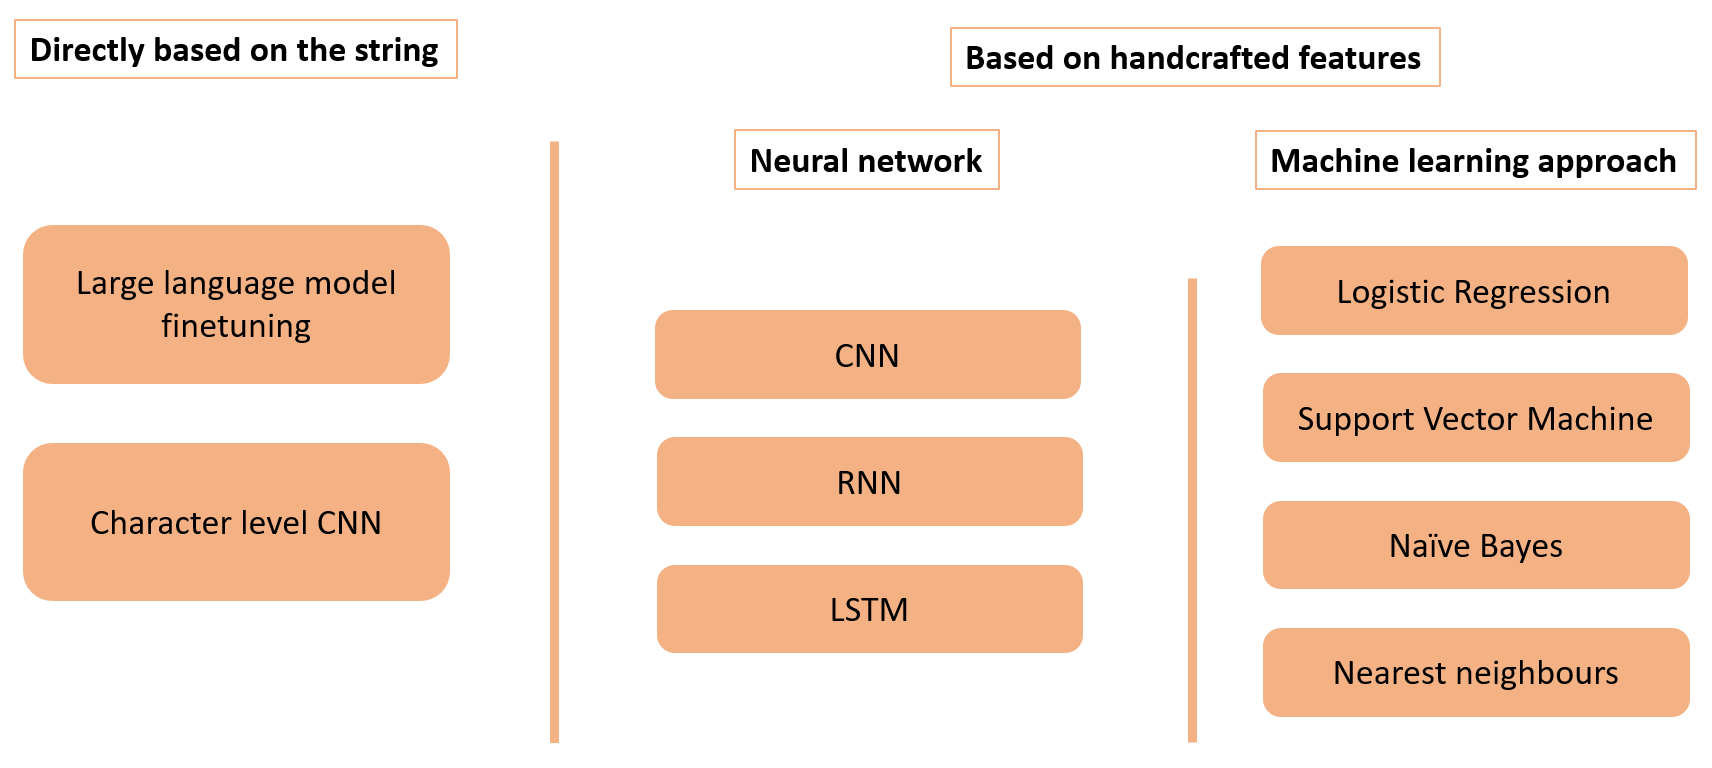
\includegraphics[width=\linewidth]{report_img/modelspresentation}
        \caption{}
        \label{fig:model_presentation}
    \end{figure}


    \subsection{Dataset}\label{sec:dataset}
    In our initial project proposal, we intended to utilize the PILU-90K~\cite{PhishingURLDetection}. However, accessing this dataset proved to be challenging due to the requirement of a formal request by a professor supervising the project. Consequently, we shifted our focus to the most extensive dataset identified in our research, specifically the one proposed in~\cite{VisualizingRNNInURLDetection}. Among the available datasets with sufficient volume for neural network model training, this particular dataset is the most recent and provides open access.

    Originally, this dataset is tailored for training Recurrent Neural Network (RNN) models, with its data already encoded in integer array formats. To adapt this dataset for broader Machine Learning applications, we undertook a preprocessing step to convert these integer arrays back into textual URL formats. Furthermore, in our exploration of neural network methodologies, we are not only utilizing the original vectorization techniques of the dataset but also experimenting with alternative vectorization strategies.

    We've thought about manually generating datasets, in case we are unable to find public datasets.
    For instance, we could extract malicious URLs from phishing e-mail datasets.
    We could also manually gather URLs from PhishTank, OpenPhish, or PhishRepo, but we expect that the few weeks that we may be able to gather URLs will not give us a large enough dataset, also considering the need for verification and the unknown project grade contribution of dataset generation.

    In addition, if we want to follow the methodology described in ~\cite{PhishingLoginURLDetection}, we would have to manually crawl hundreds of thousands of web pages using headless browsers in order to find the login page.
    We did not consider this option because of the time and resources required, especially since browsers take many resources and are hard to parallelize.
    We also expected issues with running into Web Application Firewalls when visiting so many websites, further decreasing the quality of our dataset.

    \section{Models based on handcrafted features}\label{sec:models-based-on-handcrafted-features}

    Why considering approaches that relies on handcrafted features?
    because we want to use ML techniques, not only neural networks.
    + because it enables to reduce the dimension of the data, so to have a faster treatment and analysis afterwards.
    Intuitively, the information contained by an URL should be encoded into a far smaller dimension, which is what we try to reproduce by establishing a feature vector.
    Goal for us is to reduce from one dimension for each character for the biggest URL to one dimension for each interesting information only (ideally we would like each feature to represent one base vector onto the vector space encoding the information).
    In practice, we will try to find meaningful features that brings the best possible results, so there will be information loss.
    However, we can efficiently reduce the number of dimension
    - it reduces the number of information and introduces human intervention, which is bad in general because it introduces biases or lost of information.

    \subsection{Establishment of the feature vector}\label{subsec:establishement-of-the-feature-vector}

    TTo start, we're creating a feature vector from URLs - this is our first step in using stats to identify phishing sites.
    We've picked various features based on existing research, but we've left out those that need complex language processing.
    Also, we've added some new features we thought would be useful.

    We know some of these features might overlap or be more useful than others.
    Our plan is to figure out which features are really important and then narrow them down to keep only the best ones for spotting phishing URLs.

    \subsubsection{Computations of different features}

    \begin{table}[h]
        \centering
        \begin{tabular}{|c|l|p{6cm}|c|c|l|}
            \hline
            \textbf{No.} & \textbf{Feature Name} & \textbf{Feature Description}                 & \textbf{Chi Score} & \textbf{Chi Ranking} & \textbf{Source} \\ \hline
            1            & Number of Dots        & Number of '.' in the URL                     & 64369              & 10                   &                 \\ \hline
            2            & Number of Hyphens     & Number of '-' in the URL                     & 519064             & 2                    &                 \\ \hline
            3            & Number of @           & Number of '@' in the URL                     & 4470               & 16                   &                 \\ \hline
            4            & Number of ?           & Number of '?' in the URL                     & 9005               & 13                   &                 \\ \hline
            5            & URL Length            & Length of the URL                            & 291630             & 4                    &                 \\ \hline
            6            & Number of Digits      & Number of digits in the URL                  & 312999             & 3                    &                 \\ \hline
            7            & Number of /           & Number of '/' in the URL                     & 25734              & 12                   &                 \\ \hline
            8            & Number of //          & Number of '//' in the URL                    & 194                & 21                   &                 \\ \hline
            9            & Use of HTTPS          & Counts occurrences of 'https'                & 164580             & 5                    &                 \\ \hline
            10           & Use of HTTP           & Counts occurrences of 'http'                 & 214                & 20                   &                 \\ \hline
            11           & Use of WWW            & Counts occurrences of 'www'                  & 1155               & 19                   &                 \\ \hline
            12           & IP Address Usage      & 1 if IP address is used, 0 otherwise         & 20048              & 14                   &                 \\ \hline
            13           & Suspicious Word Count & Counts suspicious words in the URL           & 518695             & 1                    &                 \\ \hline
            14           & TLD Position          & Position of Top-Level Domain in URL          & 19567              & 15                   &                 \\ \hline
            15           & Path Length Ratio     & Ratio of path length to URL length           & 64                 & 23                   &                 \\ \hline
            16           & Suspicious Char Count & Counts suspicious characters in URL          & 96471              & 9                    &                 \\ \hline
            17           & Symbol as Last Char   & 1 if last character is a symbol, 0 otherwise & 0                  & 24                   &                 \\ \hline
            18           & Redirection Count     & Counts number of '.' in subdomain            & 264180             & 6                    &                 \\ \hline
            19           & IP Address Presence   & 1 if IP address present, 0 otherwise         & 19912              & 17                   &                 \\ \hline
            20           & Subdomain Count       & Number of subdomains                         & 67397              & 11                   &                 \\ \hline
            21           & Port Presence         & 1 if port number present, 0 otherwise        & 385                & 22                   &                 \\ \hline
            22           & Unicode Char Count    & Number of unicode characters                 & 291297             & 7                    &                 \\ \hline
            23           & Query Presence        & 1 if query present in the URL, 0 otherwise   & 0                  & 25                   &                 \\ \hline
        \end{tabular}
        \caption{Summary of Features Implemented for Phishing URL Detection}
        \label{table:features}
    \end{table}

    \subsubsection{Filtering for working with the most relevant features}

    We expect some of them to be correlated, and some of them to be irrelevant.
    To improve our method in terms of computation speed as well as interpretability, we want to keep only the most relevant features.
    As provided in\cite{LexicalFeatureSelection}, we expect only a small number of features to be improve the accuracy.
    As showed on their graph below, above a threshold, the accuracy of their model do not increase anymore with the number of features used.

    \begin{figure}[H]
        \centering
        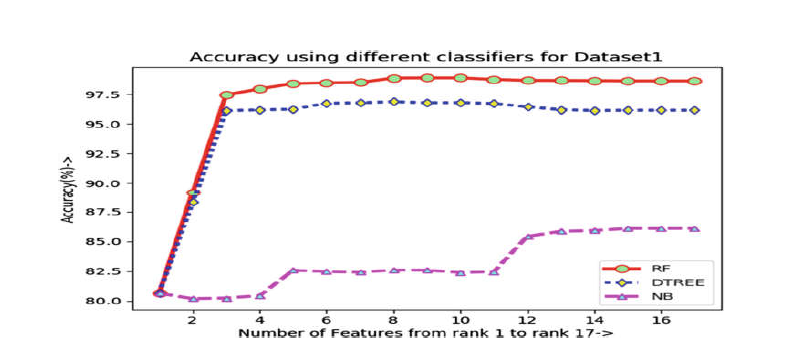
\includegraphics{report_img/lexicalfeatureselectionaccuracygraph}
        \caption{Feature wise accuracy of classifiers from\cite{LexicalFeatureSelection}}
        \label{fig:}
    \end{figure}

    Lots of different methods exist to select the most relevant features, among them
    \begin{itemize}
        \item Principal Component Analysis (PCA)
        \item Chi-Square
        \item Information Gain
        \item Anova % TODO complete with other methods
    \end{itemize}

    % TODO justify the analysis of these specific methods
    In the context of feature selection for binary classification of phishing URLs, we examined the advantages and disadvantages of Principal Component Analysis (PCA), Chi-Square, and Information Gain.

    PCA is a dimensionality reduction method.
    It is interesting in our context were numerous features may be related.
    However, we decided to discard it because:
    \begin{enumerate}
        \item we loose the interpretability of the features, which is the main motive behind handcrafted features.
        \item the encoding of a new URL for testing it is more complex, compared to feature selection.
        Therefore, we loose the practicality of the approach.
    \end{enumerate}

    We then considered Information Gain, as used in\cite{EfficientDeepLearningPhishingDetection} to feed into neural networks.
    However, we decided to discard it because:

    In the realm of binary classification for phishing URL detection, we evaluated the suitability of Principal Component Analysis (PCA), Chi-Square, and Information Gain as feature selection methods.

    PCA, known for its dimensionality reduction capabilities, initially seemed promising given the potential interrelation among numerous features.
    However, we ultimately opted against it due to two primary reasons:
    \begin{enumerate}
        \item PCA looses the interpretability of handcrafted features, which is our main motive behind handcrafted features.
        \item encoding a new URL for testing becomes markedly more complex, detracting from the method's practicality.
    \end{enumerate}

    Our attention then shifted to Information Gain, as demonstrated in\cite{EfficientDeepLearningPhishingDetection} for feeding into neural networks.
    While Information Gain excels in measuring entropy reduction and is effective with both categorical and continuous variables, it falls short in capturing the correlation between features since it assesses them in isolation.

    This led us to Chi-Square, used in\cite{LexicalFeatureSelection}, a method renowned for its effectiveness in assessing the relevance of categorical features in classification tasks.
    Chi-square score is computed using the observed and expected frequencies of the features following the formula:
    \begin{equation}
        \chi^2 = \sum \frac{(O_i - E_i)^2}{E_i}
    \end{equation}
    where \( \chi^2 \) is the Chi-Square statistic, \( O_i \) is the observed frequency, and \( E_i \) is the expected frequency under the null hypothesis that the feature and the target are independent.

    Chi-Square quantifies the independence, or lack thereof, between categorical variables and the target variable, offering a straightforward and computationally efficient approach for binary classification.

    Considering these factors, Chi-Square emerged as the most appropriate technique for our study.
    Its simplicity, efficiency, and focus on categorical feature relevance align well with the nature of our dataset and the objectives of our phishing URL classification project.


%    TODO add a graph on the influence of the number of parameters that we keep on the performance of the different models for one or several easy ML models + conclusion on the number k used afterwards

    \subsection{Implementation}\label{subsec:implementation}

    \subsubsection{Preprocessing}\label{subsubsec:preprocessing}
    Since we are building models based on both handcrafted features and on the string embedding, we need to preprocess the data differently.
    In the directory \texttt{data\textbackslash convert}, we provide a script \texttt{dill\_to\_csv.py} to convert the dill dataset from the integer array format to a textual URL format.
    The result is stored in \texttt{data\textbackslash csv\textbackslash (test/train/val).csv}.
    The other script \texttt{csv\_to\_feature\_vector.py} converts this csv from textual URL format to a feature vector using the feature selection described in \Cref{subsec:establishement-of-the-feature-vector}.
    The results are stored in \texttt{data\textbackslash feature\_vector\textbackslash (k)\textbackslash (test\_x/train\_x/val\_x).csv} where is k refers to the k in top k selected features.

    \subsubsection{Machine Learning}
    For the machine learning framework, we decided to use RAPIDS AI’s cuML over sklearn due to its significant performance advantages when dealing with large datasets.
    Leveraging the GPU, cuML achieves a 10 to 50 times speedup compared to CPU-bound libraries like sklearn.
    Unlike sklearn, which operates primarily on CPUs and can struggle with scalability, cuML is designed to handle vast amounts of data more efficiently.
    Additionally, its API mirrors that of sklearn, offering ease of use and a familiar environment for those accustomed to sklearn, but with the added benefit of GPU acceleration.
    This makes cuML an attractive choice for projects without the need for extensive adjustment to new programming paradigms.

    The framework does not provide solutions to perform hyperparameter optimization, so we picked another library called hyperopt for this.
    Hyperopt is a powerful and versatile library for hyperparameter optimization in machine learning algorithms.
    Hyperopt employs Bayesian optimization, specifically the Tree of Parzen Estimators (TPE) algorithm, which stands out for its efficiency in navigating the hyperparameter space.
    Unlike the exhaustive search approach used in sklearn's GridSearchCV or the randomness of RandomizedSearchCV, Hyperopt's method is more focused and informed, learning from each iteration to concentrate on the most promising hyperparameter combinations.
    Optuna is another library that offers similar features.
    Hyperopt was a more appropriate choice for this project due to our experience with it and its ability to serve all our hyperparameter needs.

    Since most of the tested Machine Learning algorithms are quick and require little memory, we used hyperopt's \texttt{MongoTrials} to parallelize the parameter search.
    A simple Docker Compose yaml file is provided.

    % @Jop
    % comment on speeding hyper parameter optimization, how to implement all the different models with the same frameworks, etc.
    % table with the recap of all hyper parameters, the ranges that have been tried and the best values obtained?

    \subsection{Logistic Regression}\label{subsec:logistic-regression}

    \subsubsection{Motivation of this implementation}
    We wanted to implement a simple model to have a baseline for the performance of the other models.
    Its easy implementation makes it a practical model for experimenting.
    It also provides a good interpretability of the results.

    \subsubsection{Results}

    \subsection{Support Vector Machine}\label{subsec:support-vector-machine}

    \subsubsection{Motivation of this implementation}
    Idea behind the choice of Support Vector Machine was to chose a non linear kernel, and to have a model that provides non linear decision boundaries.
    However, for optimization reasons, we chose to use a linear kernel, because it is the fastest to train on our dataset using scikit-learn, and the only available method using cumul.
    We, of course, find the same results than the linear regression, but we run it as a test to check that this implementation and linear regression are both working.

    \subsubsection{Results}

    \subsection{Naives Bayes}\label{subsec:naives-bayes}

    \subsubsection{Motivation of this implementation}

    \subsubsection{Results}

    \subsection{Nearest neighbours}\label{subsec:nearest-neigbours}

    \subsubsection{Motivation of this implementation}
    Motivation of this implementation is to have a model that provides non linear decision boundaries.

    \subsubsection{Results}

    \subsection{Recurrent neural network}\label{subsec:recurrent-neural-network}

    \subsubsection{Motivation of this implementation}

    \subsubsection{Results}

    \subsection{Convolutional neural network}\label{subsec:convolutional-neural-network}

    \subsubsection{Motivation of this implementation}

    \subsubsection{Results}

    \subsection{Long Short Term memory}\label{subsec:long-short-term-memory}

    \subsubsection{Motivation of this implementation}

    \subsubsection{Results}


    \section{Models based on the string embedding}\label{sec:models-based-on-the-string-embedding}

    \subsection{Character level convolutional neural network}\label{subsec:character-level-convolutional-neural-network}

    \subsubsection{Motivation of this implementation}

    \subsubsection{Implementation}

    \subsubsection{Results}

    \subsection{Large language model fine tuning}\label{subsec:large-language-model-finetuning}

    \subsubsection{Motivation of this implementation}

    \subsubsection{Implementation}

    \subsubsection{Results}


    \section{Conclusion}\label{sec:conclusion}
    Bla bla on the contribution that this work brings and how nice and original it is
    Further perspectives


    \bibliographystyle{plain}
    \bibliography{refs}

\end{document}